\subsection{ Fundamental Review of the Trading Book}
【背景:FRTB 是巴塞尔委员会提出的一项重要改革， 旨在修订市场风险监管资本计算方式。FRTB 提出了更复杂的方法来确定市场风险资本。最终版本的规则于 2016 年发布， 国际商定的实施日期为 2023 年 1 月， 但许多司法管辖区表示， 具体实施时间会晚一到两年。】

\subsubsection{风险计量}




\begin{itemize}
\item 巴塞尔 I 和 II.5: 市场风险计量使用 10 天， 99\%置信水平的 VaR

\item FRTB 提出: Instead of VaR with a 99 confidence level， expected shortfall (ES) with a 97.5 confidence level is proposed， actually stressed ES with a 97.5 confidence level. 【使用 97.5\%的 stressed ES】

    \begin{itemize}
    \item For normal distributions， VaR with a 99\% confidence and ES with a 97.5\% confidence are almost exactly the same. 【正常情况下，99\%的 VaR=97.5\%的 ES
    \item For non-normal distributions， they are not equivalent. When the loss distribution has a heavier tail than a normal distribution， the 97.5\% ES can be considerably greater than the \({99}\%\) VaR. 【non-normal 下， \({99}\%\) 的 VaR<97.5\%的 ES
    \end{itemize}
\end{itemize}

\subsubsection{Liquidity horizons .}
    \begin{itemize}
    \item Liquidity horizon represents the time required to sell the position or to hedge all material risks in a stressed market. 【通俗理解， liquidity horizon 是在压力市场条件下， 并且在不影响市场价格情况下， 完成交易所需要的时间】
    \item 巴塞尔 I 和 II.5: 10-day time horizon
    \item FRTB: Five different liquidity horizons are used: 10 days， 20 days， 40 days， 60 days， and 120 days. 【更真实地考虑了不同金融产品的特征】
    \end{itemize}

\subsubsection{银行交易账户的风险度量}

\begin{itemize}
\item Banking book 和 Trading Book 的分类: 确定好资产的分类， 避免监管套利。 【资产归在不同的账簿中， 计提的资本金不同】

\item FRTB: 计算市场风险资本金 market risk capital 可用 standardized approach 标准法和 internal models approach 内部模型法.【具体细节见后面】
    \begin{itemize}
    \item 理解: 站在银行的角度， 希望市场风险资本金越低越好， 因此有动力选择让资本金变低的模型， 通常最后是 internal models approach。针对这一点， 巴塞尔协议做了约束:
    \item 内部模型计算出的资本金不能过低， 不能小于标准法的 72.5\%
    % 举例
    \item \textbf{举例:} 一个银行使用 internal models approach 计算出的资本金是 100，标准法计算出的是 120。那么银行最终的资本金是 100 (因为 100 大于 120*72.5\%)
    \end{itemize}
    % FRTB与之前市场风险监管要求的区别
\item A difference between FRTB and previous market risk regulatory requirements is that most calculations are carried out at the trading desk (交易台) level.
  \begin{itemize}
    \item permission to use the internal models approach is granted on a desk-by-desk basis.
    \item 在FRTB框架下，监管要求的计算更精细，具体到每一个交易台(trading desk)。也就是说，银行不能整体申请使用内部模型，而是需要逐个交易台申请许可。
    \item \textbf{Trading desk 交易台:} 是金融机构中负责特定类型资产或金融产品交易的团队或部门。每个交易台通常专注于某一类资产，如股票、债券、外汇、衍生品等。
    \end{itemize}

\item Backtesting：FRTB 不对 stressed ES 进行回测。回测比较困难。相比之下，回测 VaR 更为简单。
  \begin{itemize}
    \item 针对 VaR 的回测建议使用一天的和最近 12 个月的数据。
    \item 如果对于 99\%VaR，出现超过 12 次异常值，或者在 97.5\%VaR 超过 30 次异常值，则必须使用 Standardized Approach 计算资本。【关于这块内容会在操作风险这个科目更详细地学习】
  \end{itemize}

\item Profit/Loss Attribution 利润/损失归因: Banks are required to compare the actual profit or loss in a day with that predicted by their models.

\item Securitizations 证券化产品
  \begin{itemize}
    \item Basel II.5 引入了 comprehensive risk measure 综合风险措施（CRM）。CRM 规则允许银行（在监管批准下）使用自己的模型，那么不同银行对同一投资组合计算的资本费用差异太大。因此，根据 FRTB，证券化产品必须使用标准化方法计算资本费用。
  \end{itemize}
\end{itemize}





\subsubsection{standardized approachh 和 internal models approach}


1） standardized approach: Capital requirement 是三个 components 的加总


\begin{center}
    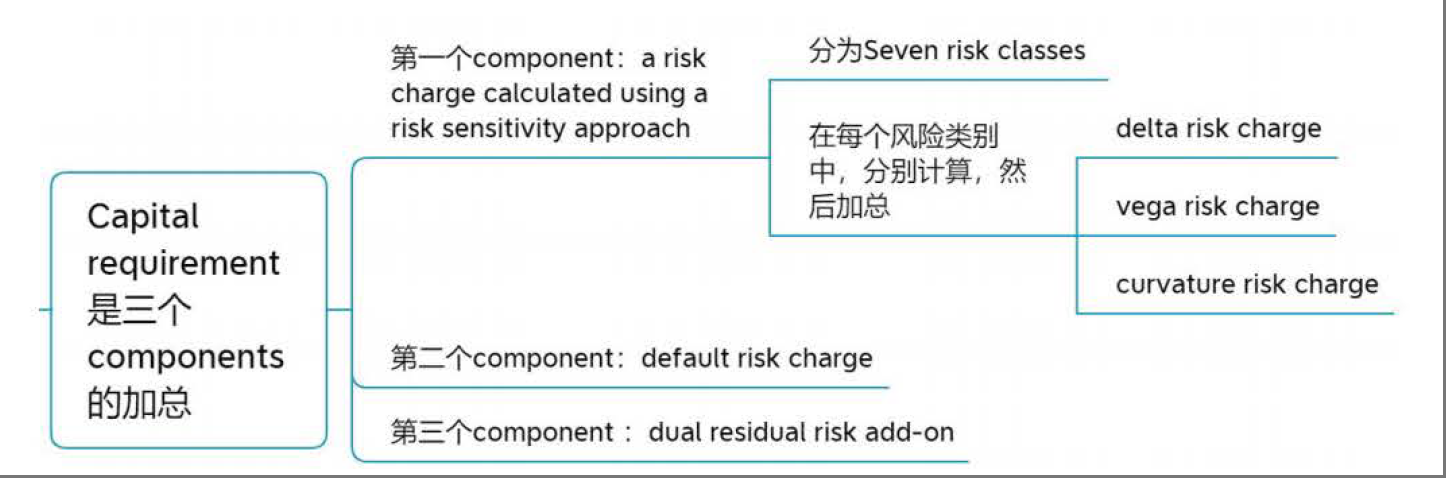
\includegraphics[width=0.4\textwidth]{images/cap.png}
    \end{center}
    \hspace*{3em} 

    
    % 详细内容
\begin{itemize}
\item 第一个 component: a risk charge calculated using a risk sensitivity approach
      \begin{itemize}
        \item Seven risk classes (对应不同的交易部门): general interest rate risk， foreign exchange risk， commodity risk， equity risk， and three categories of credit spread risk.
        \item 在每个风险类别中，计算 delta risk charge， vega risk charge， and curvature risk charge。
        \end{itemize}

        \begin{itemize}

\item[A.] The delta risk charge for a risk class is calculated using the risk weights and weighted sensitivity approach:【此公式了解即可】
        
        \[ \text{risk charge} = \sum_i \sum_j \rho_{ij}\delta_i\delta_jW_iW_j \]
        \begin{itemize}

    \item $W_i$， $W_j$: risk weights【巴塞尔委员会给定】
    \item $\rho_{ij}$: correlations between risk factors【巴塞尔委员会给定】
    \item $\delta_i$， $\delta_j$: weighted sensitivities (or deltas)【银行自己确定的delta小写的delta】
        \end{itemize}

\item 对于股票价格、汇率或商品价格等风险因素：the deltas measure the sensitivity of the portfolio to percentage changes.【delta衡量投资组合对百分比变化的敏感度。】
    \begin{itemize}
    \item 例如，如果商品价格上涨 1\% 会使投资组合价值增加 3000 美元，那么 delta 就是 300000(=3000÷0.01)。
    \end{itemize}
        
\item 对于利率和信用利差等风险因素：delta考虑的是绝对变化(absolute changes)。
    \begin{itemize}
    \item 例如，如果利率上升一个基点（0.0001）会使投资组合价值减少 200 美元，那么相对于该利率的 delta 就是 -2000000(=-200÷0.0001)。
    \end{itemize}
        
\item risk weights($W_i$) are set equal to multiples of the stressed daily volatility to reflect the liquidity horizon and the confidence level that regulators wish to consider.【risk weights=压力日波动率的倍数】
    \begin{itemize}
    \item 例如：Suppose that the stressed daily volatility of risk factor i is estimated as 2\% and that the risk factor has a 20-day liquidity horizon. $The risk weight = 0.02* 20^{0.5} *2.338 = 0.209.$ 【2.338 是 97.5\%对应的关键值→97.5\%的 stressed ES】

    \end{itemize}
\end{itemize}


\begin{itemize}

\item[B.] Vega 风险的处理方式与 delta 风险类似，但内在考虑因素不同。【回忆一级：Vega 考虑的波动率变化对于组合价值影响】
    
\item There are assumed to be \textcolor{red}{no diversification} benefits between risk factors in different risk classes and between the vega risks and delta risks within a risk class.【假定不同风险类别间的风险因素，以及同一风险类别内的 vega 风险和 delta 风险，均不存在分散化效果。】
\end{itemize}
\begin{itemize}

\item[C.] The curvature risk charge is a capital charge for a bank's \textcolor{red}{gamma risk} exposure under the standardized approach.
    
\item 第二个 component: default risk charge
    \begin{itemize}
    \item FRTB 将信用风险影响分为两类：
        \begin{itemize}
        \item Credit spread risk (信用利差风险): 指公司的信用利差发生变化带来的风险。【不一定违约】
            
            \item 风险计量方式和市场风险(delta/vega/curvature approach)一样【因为信用利差的变动会像其他市场风险因素一样，对投资组合的价值产生影响】
            
        \item Default risks(Jump-to-default risk 跳至违约风险): 指公司可能发生违约的风险。
            
            \item Default risks are handled by a \textcolor{red}{separate default risk charge}.
            \item default risk charge = each exposure * loss given default (LGD) * default risk weight
            \item LGD 和 risk weight 由 Basel Committee 设定.
            \item For example， the LGD for senior debt is specified as 75\% and the default risk for a counterparty rated A is 3\%.
            \item Equity positions are subject to a default risk charge with an LGD = 100\%.
            \item Rules for \textcolor{red}{offsetting exposures} are specified. 【允许银行在符合一定条件的情况下，对不同的风险敞口进行相互抵消，更准确地反映实际面临的违约风险。】
        \end{itemize}

        \end{itemize}
    \end{itemize}
    
\item 第三个 component: dual residual risk add-on
    \begin{itemize}
    \item Residual risk add-on 剩余风险附加费：主要考虑前面 delta/vega/curvature 方法无法处理的风险。
        \begin{itemize}
        \item 比如奇异期权
        \end{itemize}
    \end{itemize}

\item 其他：
    \begin{itemize}
    \item 一般是一些大银行使用 standardized approach；
    \item 小银行可以使用简化的 standardized approach → Simplified Approach(比如不考虑 vega and gamma risk)
    \end{itemize}
    
\item[2] internal models approach 内部模型法→历史模拟法
    \begin{itemize}
    \item 估计 97.5\% stressed ES。
        \item FRTB 并未规定具体的计算方法，通常会使用\textcolor{red}{历史模拟法 historical simulation approach}。
        \item In Basel I and Basel II.5， banks are allowed to deduce the impact of 10-day changes from the impact of one-day changes using a $\sqrt{10}$ multiplier.
        \item In \textcolor{red}{FRTB}， banks are required to consider changes over periods of \textcolor{red}{10 days} that occurred \textcolor{red}{during a stressed period in the past}.
        \item 注意：
            \begin{itemize}
            \item 计量经济学家主张：时间是非重叠的 non-overlapping periods，因为希望观测值是独立的
            \item FRTB 认为时间是重叠的也可以的 overlapping periods【更符合实际情况】
            \end{itemize}
        \item \textcolor{red}{liquidity-adjusted ES}：考虑了不同风险因素流动性期限差异后的 ES.【公式不需要掌握，知道大概意义。公式的推导过程略】
    
    \[ \text{liquidity-adjusted ES} = \sqrt{ES_1^2 + \sum_{i=2}^5 (ES_i\sqrt{\frac{LH_i-LH_{i-1}}{10}})^2} \]
        \begin{itemize}
        \item LH: liquidity horizon 【在前面已介绍，分为 5 种，10 天、20 天等】
        \end{itemize}
    \item 这个公式的推导叫做 cascade approach，同样也可用于计算 VaR。
    \end{itemize}
\end{itemize}














%\begin{example}{例子}
 %   例子例子例子
%\end{example}

%\begin{boxa}{例子}
 %   例子例子例子
%\end{boxa}

%\begin{knowledgebox}{例子}
 %   例子例子例子
%\end{knowledgebox}



%\begin{skillbox}{例子}
 %   例子例子例子
%\end{skillbox}

%\begin{theorembox}{例子}
 %   例子例子例子
%\end{theorembox}


%\begin{note}{例子}
%    例子例子例子
%\end{note}
